%=============================================================
% Smart Bank AI — Rapport de Projet Encadré
% INSEA 2025-2026
% Auteurs : Amina Bajdouri, Oumaima Belbaraka
%=============================================================
\documentclass[12pt,a4paper]{report}

%--------------------------------------------------------------
% Packages
%--------------------------------------------------------------
\usepackage[utf8]{inputenc}
\usepackage[T1]{fontenc}
\usepackage[french]{babel}
\usepackage{graphicx}
\usepackage{float}
\usepackage{geometry}
\usepackage{hyperref}
\usepackage{xcolor}
\usepackage{booktabs}
\usepackage{array}
\usepackage{longtable}
\usepackage{listings}
\usepackage{fancyhdr}
\usepackage{titlesec}
\usepackage{setspace}
\usepackage{microtype}
\usepackage{amsmath}
\usepackage{amssymb}
\usepackage{caption}
\usepackage{subcaption}
\usepackage{enumitem}
\usepackage{mdframed}
\usepackage{tabularx}
\usepackage{multirow}
\usepackage{lmodern}
\usepackage{pifont}

%--------------------------------------------------------------
% Mise en page
%--------------------------------------------------------------
\geometry{
  a4paper,
  top=2.5cm,
  bottom=2.5cm,
  left=3cm,
  right=2.5cm,
  headheight=15pt
}

\setstretch{1.2}

%--------------------------------------------------------------
% Couleurs
%--------------------------------------------------------------
\definecolor{insea-blue}{RGB}{0,74,128}
\definecolor{insea-green}{RGB}{0,128,96}
\definecolor{code-bg}{RGB}{245,245,245}
\definecolor{code-kw}{RGB}{0,0,180}
\definecolor{code-str}{RGB}{163,21,21}
\definecolor{code-cmt}{RGB}{0,128,0}
\definecolor{mygreen}{RGB}{0,128,64}

%--------------------------------------------------------------
% Style des titres de chapitres
%--------------------------------------------------------------
\titleformat{\chapter}[display]
  {\normalfont\huge\bfseries\color{insea-blue}}
  {\chaptertitlename\ \thechapter}{20pt}{\Huge}
\titlespacing*{\chapter}{0pt}{30pt}{40pt}

%--------------------------------------------------------------
% En-têtes et pieds de page
%--------------------------------------------------------------
\pagestyle{fancy}
\fancyhf{}
\fancyhead[L]{\small\textit{Smart Bank AI}}
\fancyhead[R]{\small\textit{Projet Encadré — INSEA 2025-2026}}
\fancyfoot[C]{\thepage}
\renewcommand{\headrulewidth}{0.4pt}

%--------------------------------------------------------------
% Style listings (code source)
%--------------------------------------------------------------
\lstdefinestyle{python}{
  language=Python,
  backgroundcolor=\color{code-bg},
  basicstyle=\ttfamily\small,
  keywordstyle=\color{code-kw}\bfseries,
  stringstyle=\color{code-str},
  commentstyle=\color{code-cmt}\itshape,
  numberstyle=\tiny\color{gray},
  breakatwhitespace=false,
  breaklines=true,
  captionpos=b,
  numbers=left,
  stepnumber=1,
  showstringspaces=false,
  frame=single,
  rulecolor=\color{gray!40},
  tabsize=4,
  xleftmargin=1.5em
}

\lstdefinestyle{bash}{
  language=bash,
  backgroundcolor=\color{code-bg},
  basicstyle=\ttfamily\small,
  keywordstyle=\color{code-kw},
  stringstyle=\color{code-str},
  commentstyle=\color{code-cmt}\itshape,
  breaklines=true,
  frame=single,
  rulecolor=\color{gray!40},
  xleftmargin=1.5em
}

%--------------------------------------------------------------
% Hyperref
%--------------------------------------------------------------
\hypersetup{
  colorlinks=true,
  linkcolor=insea-blue,
  citecolor=insea-green,
  urlcolor=insea-blue,
  pdftitle={Smart Bank AI — Rapport de Projet Encadré},
  pdfauthor={Amina Bajdouri, Oumaima Belbaraka},
  pdfsubject={INSEA Projet Encadré 2025-2026}
}

%--------------------------------------------------------------
% Commandes utilitaires
%--------------------------------------------------------------
\newcommand{\keyword}[1]{\textbf{#1}}
\newcommand{\techterm}[1]{\textit{#1}}

%==============================================================
\begin{document}
%==============================================================

%--------------------------------------------------------------
% Page de garde
%--------------------------------------------------------------
\begin{titlepage}
  \thispagestyle{empty}
  \begin{center}
    % Logo
    \vspace*{0.5cm}
    \begin{figure}[H]
      \centering
      \includegraphics[width=0.35\textwidth]{images/logo_insea.png}
    \end{figure}

    \vspace{0.3cm}
    {\large \textbf{Institut National de Statistique et d'Économie Appliquée}}\\[0.2cm]
    {\large INSEA — Rabat, Maroc}\\[0.1cm]
    {\normalsize Année académique 2025–2026}

    \vspace{0.8cm}
    \noindent\rule{\textwidth}{1.5pt}
    \vspace{0.4cm}

    {\LARGE \textbf{Projet Encadré}}\\[0.5cm]

    {\large \textbf{\color{insea-blue}
      Application Intelligente d'Analyse des Transactions Bancaires\\
      pour la Segmentation des Dépenses\\
      et l'Aide à la Décision Budgétaire
    }}

    \vspace{0.4cm}
    \noindent\rule{\textwidth}{1.5pt}

    \vspace{1cm}
    {\large \textbf{Smart Bank AI}}\\[0.3cm]
    {\normalsize
      \textit{Analyse automatique · Catégorisation ML · Détection d'anomalies · Recommandations budgétaires}
    }

    \vfill

    \begin{minipage}[t]{0.48\textwidth}
      \textbf{Réalisé par :}\\[0.2cm]
      Amina \textsc{Bajdouri}\\
      Oumaima \textsc{Belbaraka}
    \end{minipage}
    \hfill
    \begin{minipage}[t]{0.48\textwidth}
      \raggedleft
      \textbf{Encadrante :}\\[0.2cm]
      Mme Imane \textsc{Chlioui}\\
      Professeure à l'INSEA
    \end{minipage}

    \vspace{1.5cm}
    {\small \url{https://github.com/Oumaimbk/-smart-bank-ai}}
  \end{center}
\end{titlepage}

%--------------------------------------------------------------
% Remerciements
%--------------------------------------------------------------
\chapter*{Remerciements}
\addcontentsline{toc}{chapter}{Remerciements}
\thispagestyle{fancy}

Nous tenons à exprimer notre profonde gratitude à toutes les personnes
qui ont contribué, de près ou de loin, à la réalisation de ce projet.

En premier lieu, nos remerciements les plus sincères vont à notre
encadrante, \textbf{Mme Imane Chlioui}, dont les conseils avisés, la
disponibilité et l'accompagnement bienveillant tout au long de ce projet
nous ont été d'une valeur inestimable. Ses orientations pertinentes ont
guidé nos choix techniques et académiques à chaque étape du développement.

Nous remercions également l'ensemble du corps enseignant de l'INSEA pour
la qualité de la formation dispensée tout au long de notre cursus, qui nous
a fourni les bases théoriques et pratiques nécessaires à la concrétisation
de ce projet.

Nos remerciements vont aussi aux membres de nos familles respectives pour
leur soutien moral constant et leur patience au quotidien.

Enfin, nous remercions la communauté open-source pour les outils, bibliothèques
et frameworks qui ont rendu ce projet possible.

\vspace{2cm}
\begin{flushright}
\textit{Amina Bajdouri \& Oumaima Belbaraka}\\
\textit{Rabat, 2026}
\end{flushright}

%--------------------------------------------------------------
% Résumé / Abstract
%--------------------------------------------------------------
\chapter*{Résumé}
\addcontentsline{toc}{chapter}{Résumé}
\thispagestyle{fancy}

\section*{Résumé (français)}

Dans un contexte où la gestion des finances personnelles devient un enjeu
croissant pour les particuliers, les outils intelligents capables d'analyser
automatiquement les flux bancaires représentent une valeur ajoutée considérable.
Ce rapport présente \textbf{Smart Bank AI}, une application web full-stack
dédiée à l'analyse automatisée des transactions bancaires marocaines.

L'application repose sur une architecture en trois couches : une API REST
sécurisée (Django REST Framework + JWT), un moteur de services métier, et
un pipeline d'intelligence artificielle composé de trois modèles distincts.
Le premier modèle, basé sur TF-IDF et la Régression Logistique, catégorise
automatiquement les transactions en 12 catégories avec une précision de
\textbf{99{,}6\%}. Le deuxième modèle, Isolation Forest, détecte les
comportements financiers anormaux de manière non supervisée. Le troisième,
une forêt aléatoire (Random Forest Regressor), prévoit les dépenses du mois
suivant par catégorie avec un coefficient de détermination \(R^2 = 0{,}98\).

Un moteur de recommandations génère ensuite des conseils budgétaires
personnalisés en combinant les résultats des trois modèles. L'ensemble de
la solution est conteneurisée via Docker Compose et validée par une suite
de 63 tests automatisés. Le frontend, développé en React/Vite, offre un
tableau de bord interactif avec visualisations dynamiques.

\vspace{0.5cm}
\textbf{Mots-clés :} Machine Learning, Transactions bancaires, Catégorisation,
Détection d'anomalies, Prévision, Django REST Framework, React, Docker, TF-IDF,
Isolation Forest, Random Forest, API REST, JWT.

\section*{Abstract (English)}

In a context where personal finance management is an increasing challenge
for individuals, intelligent tools capable of automatically analysing
banking flows represent significant added value. This report presents
\textbf{Smart Bank AI}, a full-stack web application dedicated to the
automated analysis of Moroccan banking transactions.

The application is built on a three-layer architecture: a secure REST API
(Django REST Framework with JWT authentication), a business service layer,
and an artificial intelligence pipeline comprising three distinct models.
The first model, based on TF-IDF and Logistic Regression, automatically
categorises transactions into 12 categories with an accuracy of
\textbf{99.6\%}. The second model, Isolation Forest, detects abnormal
financial behaviour in an unsupervised manner. The third, a Random Forest
Regressor, predicts next-month expenses by category with a coefficient of
determination \(R^2 = 0.98\).

A recommendation engine then generates personalised budgetary advice by
combining the results of all three models. The entire solution is
containerised via Docker Compose and validated by a suite of 63 automated
tests. The frontend, developed in React/Vite, provides an interactive
dashboard with dynamic visualisations.

\vspace{0.5cm}
\textbf{Keywords:} Machine Learning, Banking transactions, Categorisation,
Anomaly detection, Forecasting, Django REST Framework, React, Docker, TF-IDF,
Isolation Forest, Random Forest, REST API, JWT.

%--------------------------------------------------------------
% Tables des matières / figures / tableaux
%--------------------------------------------------------------
\tableofcontents
\listoffigures
\listoftables

%==============================================================
\chapter{Introduction générale}
%==============================================================

\section{Contexte et motivation}

La révolution numérique a profondément transformé les habitudes bancaires.
Aujourd'hui, l'immense majorité des transactions financières — virements,
paiements par carte, retraits — laissent une trace numérique exploitable.
Pourtant, la plupart des particuliers peinent à tirer parti de cette mine
d'informations : les relevés bancaires bruts ne permettent guère d'identifier
les tendances de consommation, de repérer des dépenses inhabituelles, ni
de planifier l'avenir budgétaire.

Au Maroc, le secteur bancaire connaît une numérisation accélérée portée par
des initiatives telles que Bank Al-Maghrib et les stratégies d'inclusion
financière. Des millions de transactions sont générées quotidiennement, mais
les outils d'analyse personnels restent peu répandus et souvent peu adaptés
aux spécificités du marché marocain (nomenclature des commerçants, services
locaux, langues mélangées dans les libellés).

C'est dans ce contexte que s'inscrit \textbf{Smart Bank AI} : une application
web intelligente qui transforme un simple fichier CSV de transactions bancaires
en un tableau de bord analytique complet, enrichi par des modèles de machine
learning entraînés sur des données marocaines.

\section{Problématique}

La gestion des finances personnelles soulève plusieurs problèmes fondamentaux
pour l'utilisateur non averti :

\begin{itemize}[noitemsep]
  \item \textbf{Catégorisation manuelle fastidieuse :} classer chaque transaction
    (alimentation, transport, loisirs…) représente un effort considérable et est
    source d'erreurs.
  \item \textbf{Détection tardive des anomalies :} les débits inhabituels
    (montants suspects, horaires atypiques, fréquences anormales) passent souvent
    inaperçus jusqu'à la fin du mois.
  \item \textbf{Absence de vision prospective :} sans outil d'aide à la décision,
    il est difficile d'anticiper les dépenses du mois suivant et d'adapter son
    comportement budgétaire.
  \item \textbf{Manque de personnalisation :} les recommandations génériques
    n'ont que peu d'utilité ; seule une analyse des données propres à chaque
    utilisateur peut produire des conseils pertinents.
\end{itemize}

Ces constats soulèvent la question centrale suivante : \textit{Comment exploiter
les données transactionnelles bancaires pour fournir, de manière automatique et
personnalisée, une analyse complète de la situation financière d'un utilisateur
et des recommandations actionnables ?}

\section{Objectifs du projet}

Ce projet vise à concevoir et réaliser une application répondant aux objectifs
suivants :

\begin{enumerate}[noitemsep]
  \item \textbf{Catégoriser automatiquement} les transactions bancaires en
    12 catégories via un pipeline de machine learning.
  \item \textbf{Détecter les anomalies financières} de manière non supervisée
    et en temps réel lors de l'import des données.
  \item \textbf{Prévoir les dépenses futures} par catégorie pour le mois suivant.
  \item \textbf{Générer des recommandations budgétaires} personnalisées basées
    sur les données historiques et les anomalies détectées.
  \item \textbf{Sécuriser les données} de chaque utilisateur via une
    authentification JWT et un cloisonnement strict des accès.
  \item \textbf{Offrir un tableau de bord interactif} permettant d'explorer
    les données sous différents angles analytiques.
\end{enumerate}

\section{Plan du rapport}

Ce rapport est organisé en six chapitres :

\begin{itemize}[noitemsep]
  \item \textbf{Chapitre 2 — Analyse et spécification des besoins :}
    étude de l'existant, identification des besoins fonctionnels et non
    fonctionnels, acteurs et cas d'utilisation.
  \item \textbf{Chapitre 3 — Conception :} architecture globale,
    diagrammes de classes et de séquences, conception de la base de données.
  \item \textbf{Chapitre 4 — Module d'Intelligence Artificielle :}
    description détaillée des trois modèles ML et du moteur de recommandations.
  \item \textbf{Chapitre 5 — Réalisation et implémentation :}
    technologies utilisées, déploiement Docker, backend et frontend.
  \item \textbf{Chapitre 6 — Tests et validation :}
    stratégie de test et résultats des 63 tests automatisés.
  \item \textbf{Conclusion et perspectives :} bilan, limites et pistes d'amélioration.
\end{itemize}

%==============================================================
\chapter{Analyse et spécification des besoins}
%==============================================================

\section{Étude de l'existant}

Plusieurs solutions existent sur le marché pour la gestion des finances
personnelles. Leur analyse permet d'identifier les manques auxquels
Smart Bank AI répond.

\begin{table}[H]
  \centering
  \caption{Comparaison des solutions existantes de gestion financière personnelle}
  \label{tab:comparaison-existant}
  \renewcommand{\arraystretch}{1.3}
  \begin{tabularx}{\textwidth}{>{\bfseries}lXXX}
    \toprule
    Solution & Catégorisation & Anomalies & Adapté Maroc \\
    \midrule
    Intuit Mint & Règles manuelles & Non & Non \\
    YNAB & Manuelle & Non & Non \\
    Bankin' & Partiellement ML & Basique & Partiel \\
    Banques marocaines & Absente & Absente & Oui \\
    \textbf{Smart Bank AI} & \textbf{ML (99,6\%)} & \textbf{Isolation Forest} & \textbf{Oui} \\
    \bottomrule
  \end{tabularx}
\end{table}

Les solutions existantes présentent des lacunes importantes pour le marché
marocain : elles ne gèrent pas les libellés en arabe ou en français mélangé,
ne sont pas intégrées aux relevés CSV des banques marocaines, et n'offrent
pas de détection d'anomalies basée sur des algorithmes non supervisés.

\section{Acteurs du système}

Le système fait intervenir deux types d'acteurs :

\begin{itemize}[noitemsep]
  \item \textbf{L'utilisateur authentifié :} personne physique qui importe ses
    relevés CSV, consulte son tableau de bord et ses analyses personnalisées.
    C'est l'acteur principal du système.
  \item \textbf{Le système ML (acteur secondaire interne) :} le pipeline
    d'intelligence artificielle déclenché automatiquement à chaque import
    CSV pour produire les catégories, anomalies, prévisions et recommandations.
\end{itemize}

\section{Besoins fonctionnels}

Les besoins fonctionnels ont été regroupés en six domaines :

\subsection{Gestion des comptes utilisateurs}
\begin{itemize}[noitemsep]
  \item \textbf{BF01} — L'utilisateur peut créer un compte avec email, nom d'utilisateur et mot de passe.
  \item \textbf{BF02} — L'utilisateur peut s'authentifier et obtenir un jeton JWT.
  \item \textbf{BF03} — Le jeton d'accès est rafraîchi automatiquement par le frontend.
  \item \textbf{BF04} — Chaque utilisateur n'a accès qu'à ses propres données.
\end{itemize}

\subsection{Import et traitement des données}
\begin{itemize}[noitemsep]
  \item \textbf{BF05} — L'utilisateur peut importer un fichier CSV de transactions bancaires.
  \item \textbf{BF06} — Le système valide le format du fichier (colonnes requises : \texttt{transaction\_id}, \texttt{transaction\_date}, \texttt{direction}, \texttt{amount}).
  \item \textbf{BF07} — Les doublons (même \texttt{transaction\_id} pour un même utilisateur) sont détectés et ignorés.
  \item \textbf{BF08} — L'utilisateur peut consulter l'historique de ses imports et supprimer un lot.
  \item \textbf{BF09} — La taille des fichiers est limitée à 10 Mo.
\end{itemize}

\subsection{Catégorisation des transactions}
\begin{itemize}[noitemsep]
  \item \textbf{BF10} — Chaque transaction est automatiquement assignée à l'une des 12 catégories.
  \item \textbf{BF11} — Un score de confiance est associé à chaque prédiction.
  \item \textbf{BF12} — Une approche hybride règles + ML est utilisée pour les cas simples.
\end{itemize}

\subsection{Détection d'anomalies}
\begin{itemize}[noitemsep]
  \item \textbf{BF13} — Le système détecte automatiquement les transactions anormales.
  \item \textbf{BF14} — Chaque anomalie est typée (montant élevé, heure inhabituelle, etc.).
  \item \textbf{BF15} — L'utilisateur peut consulter la liste de ses anomalies avec les détails.
\end{itemize}

\subsection{Prévisions et recommandations}
\begin{itemize}[noitemsep]
  \item \textbf{BF16} — Le système prédit les dépenses du mois suivant par catégorie.
  \item \textbf{BF17} — Des recommandations budgétaires personnalisées sont générées.
  \item \textbf{BF18} — Chaque recommandation est typée et priorisée.
\end{itemize}

\subsection{Tableau de bord analytique}
\begin{itemize}[noitemsep]
  \item \textbf{BF19} — L'utilisateur visualise ses KPIs (total dépenses, revenus, épargne nette, nb transactions).
  \item \textbf{BF20} — Un graphique en camembert présente la répartition des dépenses par catégorie.
  \item \textbf{BF21} — Un graphique en barres présente l'évolution mensuelle des flux.
  \item \textbf{BF22} — Le Top 10 des commerçants est affiché.
  \item \textbf{BF23} — L'utilisateur peut filtrer et rechercher ses transactions.
\end{itemize}

\section{Besoins non fonctionnels}

\begin{table}[H]
  \centering
  \caption{Besoins non fonctionnels de l'application}
  \label{tab:bnf}
  \renewcommand{\arraystretch}{1.3}
  \begin{tabularx}{\textwidth}{>{\bfseries}lX}
    \toprule
    Catégorie & Exigence \\
    \midrule
    Sécurité & Authentification JWT, isolation stricte des données par utilisateur,
               protection CORS, aucune donnée sensible exposée en clair \\
    Performance & Traitement d'un fichier de 2 000 transactions en moins de 10 secondes \\
    Disponibilité & Architecture conteneurisée Docker garantissant la portabilité
                    et la reproductibilité de l'environnement \\
    Fiabilité & 63 tests automatisés couvrant les unités et l'intégration ;
                détection des doublons garantie \\
    Maintenabilité & Architecture en couches séparées, code documenté,
                     pipeline ML modulaire et extensible \\
    Ergonomie & Interface responsive, visualisations interactives,
                navigation fluide entre les sections \\
    Portabilité & Application conteneurisée, déployable sur tout système
                  supportant Docker Compose \\
    \bottomrule
  \end{tabularx}
\end{table}

\section{Diagramme de cas d'utilisation}

\begin{figure}[H]
  \centering
  % CAPTURE À FAIRE: diagramme_usecase.png
  % Créer un diagramme UML de cas d'utilisation avec:
  % - Acteur "Utilisateur" à gauche
  % - Use cases: S'inscrire, Se connecter, Importer CSV,
  %   Consulter tableau de bord, Consulter transactions,
  %   Consulter anomalies, Consulter recommandations,
  %   Supprimer un lot
  % - Relations include/extend appropriées
  \includegraphics[width=0.85\textwidth]{images/diagramme_usecase.png}
  \caption{Diagramme de cas d'utilisation de Smart Bank AI}
  \label{fig:usecase}
\end{figure}

%==============================================================
\chapter{Conception}
%==============================================================

\section{Architecture globale}

Smart Bank AI est conçu selon une architecture en \textbf{trois couches}
clairement séparées, ce qui garantit la maintenabilité, la testabilité et
l'évolutivité de l'application.

\begin{figure}[H]
  \centering
  % CAPTURE À FAIRE: architecture_3couches.png
  % Schéma montrant les 3 couches verticales:
  % [Frontend React] → [API Django REST] → [Service Layer] → [ML Pipeline]
  % Avec PostgreSQL en bas et Docker Compose comme enveloppe externe
  \includegraphics[width=0.92\textwidth]{images/architecture_3couches.png}
  \caption{Architecture en trois couches de Smart Bank AI}
  \label{fig:architecture}
\end{figure}

\subsection{Couche présentation — Frontend React}

Le frontend est développé avec \textbf{React 18} et \textbf{Vite} comme
outil de build. Il communique exclusivement avec le backend via des appels
HTTP à l'API REST, en incluant un jeton JWT dans chaque requête. Les
visualisations sont produites par la bibliothèque \textbf{Recharts}.

La couche présentation comprend huit pages principales :
\begin{itemize}[noitemsep]
  \item \textbf{Login / Register :} gestion de l'authentification.
  \item \textbf{Dashboard :} KPIs, graphiques de répartition et d'évolution.
  \item \textbf{Upload :} import CSV et historique des lots.
  \item \textbf{Transactions :} tableau paginé avec filtres et recherche.
  \item \textbf{Anomalies :} liste des transactions suspectes.
  \item \textbf{Recommandations :} conseils budgétaires personnalisés.
  \item \textbf{AI Insights :} métriques d'évaluation des modèles ML.
\end{itemize}

\subsection{Couche API — Django REST Framework}

L'API REST expose des endpoints sécurisés regroupés en cinq modules :

\begin{table}[H]
  \centering
  \caption{Endpoints REST de l'application}
  \label{tab:endpoints}
  \renewcommand{\arraystretch}{1.3}
  \begin{tabularx}{\textwidth}{lllX}
    \toprule
    Module & Méthode & Endpoint & Description \\
    \midrule
    Auth & POST & \texttt{/api/auth/register/} & Inscription \\
    Auth & POST & \texttt{/api/auth/login/} & Connexion (JWT) \\
    Auth & GET & \texttt{/api/auth/me/} & Profil utilisateur \\
    Transactions & GET & \texttt{/api/transactions/} & Liste paginée \\
    Transactions & POST & \texttt{/api/transactions/upload/} & Import CSV \\
    Transactions & DELETE & \texttt{/api/transactions/batches/\{id\}/delete/} & Suppression lot \\
    Analytics & GET & \texttt{/api/analytics/kpi/} & KPIs \\
    Analytics & GET & \texttt{/api/analytics/spending-by-category/} & Répartition \\
    Analytics & GET & \texttt{/api/analytics/monthly-evolution/} & Évolution \\
    Analytics & GET & \texttt{/api/analytics/top-merchants/} & Top commerçants \\
    Anomalies & GET & \texttt{/api/anomalies/} & Liste anomalies \\
    Recos & GET & \texttt{/api/recommendations/} & Recommandations \\
    Recos & GET & \texttt{/api/recommendations/predictions/} & Prévisions \\
    ML & GET & \texttt{/api/analytics/ml-metrics/} & Métriques ML \\
    \bottomrule
  \end{tabularx}
\end{table}

\subsection{Couche service — PipelineService}

La couche service constitue le cœur métier de l'application. La classe
\texttt{PipelineService} orchestre le flux de traitement complet lors d'un
import CSV, en appelant successivement :

\begin{enumerate}[noitemsep]
  \item \texttt{load\_csv()} — lecture et validation du fichier
  \item \texttt{clean()} — nettoyage et normalisation des données
  \item \texttt{feature\_engineering()} — enrichissement des features
  \item \texttt{classify()} — catégorisation par TF-IDF + LR
  \item \texttt{detect\_anomalies()} — Isolation Forest
  \item \texttt{predict\_next\_month()} — Random Forest
  \item \texttt{generate\_recommendations()} — moteur de recommandations
  \item Persistence en base PostgreSQL via Django ORM
\end{enumerate}

\section{Diagramme de classes}

\begin{figure}[H]
  \centering
  % CAPTURE À FAIRE: diagramme_classes.png
  % Diagramme UML de classes avec les entités:
  % User (id, username, email, password)
  % Transaction (id, user_fk, transaction_id, date, amount, direction,
  %              narration, merchant_name, category, batch_fk)
  % UploadBatch (id, user_fk, filename, created_at, transaction_count)
  % Anomaly (id, transaction_fk, anomaly_type, score, details)
  % Recommendation (id, user_fk, type, message, priority, created_at)
  % Prediction (id, user_fk, category, predicted_amount, month)
  % Relations: User 1—* Transaction, Transaction 1—* Anomaly,
  %            User 1—* Recommendation, User 1—* Prediction,
  %            UploadBatch 1—* Transaction
  \includegraphics[width=\textwidth]{images/diagramme_classes.png}
  \caption{Diagramme de classes UML du modèle de données}
  \label{fig:classes}
\end{figure}

\section{Diagramme de séquence — Import CSV}

\begin{figure}[H]
  \centering
  % CAPTURE À FAIRE: diagramme_sequence.png
  % Diagramme de séquence pour le cas d'utilisation "Importer CSV":
  % Acteurs: Utilisateur, Frontend (React), Backend (API), PipelineService, ML Pipeline, PostgreSQL
  % Séquence:
  % 1. Utilisateur sélectionne fichier CSV
  % 2. Frontend POST /api/transactions/upload/ avec Bearer token
  % 3. API valide JWT, appelle PipelineService.run()
  % 4. Pipeline: load_csv → clean → classify → detect_anomalies → predict → recommend
  % 5. Résultats sauvegardés en PostgreSQL
  % 6. API retourne JSON: {new_transactions, anomalies_detected, recommendations_generated}
  % 7. Frontend affiche résultats
  \includegraphics[width=\textwidth]{images/diagramme_sequence.png}
  \caption{Diagramme de séquence — Import CSV et traitement ML}
  \label{fig:sequence}
\end{figure}

\section{Conception de la base de données}

\subsection{Entités et attributs}

La base de données PostgreSQL comprend six tables principales :

\paragraph{Table \texttt{users}}
Gère les comptes utilisateurs (fournie par le modèle \texttt{AbstractUser} de Django).
Attributs : \texttt{id} (PK), \texttt{username}, \texttt{email} (unique),
\texttt{password} (hashé bcrypt), \texttt{date\_joined}, \texttt{is\_active}.

\paragraph{Table \texttt{upload\_batches}}
Trace chaque import CSV effectué par un utilisateur.
Attributs : \texttt{id} (PK), \texttt{user\_id} (FK), \texttt{filename},
\texttt{created\_at}, \texttt{transaction\_count},
\texttt{new\_count}, \texttt{skipped\_count}.

\paragraph{Table \texttt{transactions}}
Stocke les transactions après traitement par le pipeline.
Attributs : \texttt{id} (PK), \texttt{user\_id} (FK), \texttt{batch\_id} (FK),
\texttt{transaction\_id} (identifiant unique CSV), \texttt{transaction\_date},
\texttt{direction} (\texttt{Debit}/\texttt{Credit}), \texttt{amount},
\texttt{narration}, \texttt{merchant\_name}, \texttt{category},
\texttt{category\_confidence}, \texttt{balance\_after}.
Contrainte d'unicité : (\texttt{user\_id}, \texttt{transaction\_id}).

\paragraph{Table \texttt{anomalies}}
Enregistre chaque anomalie détectée sur une transaction.
Attributs : \texttt{id} (PK), \texttt{transaction\_id} (FK),
\texttt{anomaly\_type} (\texttt{high\_amount}, \texttt{odd\_hour},
\texttt{isolation\_forest}, etc.),
\texttt{score}, \texttt{details} (JSON).

\paragraph{Table \texttt{recommendations}}
Stocke les recommandations générées pour chaque utilisateur.
Attributs : \texttt{id} (PK), \texttt{user\_id} (FK),
\texttt{rec\_type}, \texttt{message}, \texttt{priority},
\texttt{category}, \texttt{created\_at}.

\paragraph{Table \texttt{predictions}}
Contient les prévisions de dépenses par catégorie.
Attributs : \texttt{id} (PK), \texttt{user\_id} (FK),
\texttt{category}, \texttt{predicted\_amount}, \texttt{month}.

\subsection{Modèle logique des données (MLD)}

\begin{figure}[H]
  \centering
  % CAPTURE À FAIRE: mld_base_donnees.png
  % Schéma du MLD avec les 6 tables et leurs clés primaires/étrangères:
  % users (id PK, username, email, password, date_joined)
  % upload_batches (id PK, user_id FK→users, filename, created_at, transaction_count)
  % transactions (id PK, user_id FK→users, batch_id FK→upload_batches,
  %               transaction_id, transaction_date, direction, amount,
  %               narration, merchant_name, category, category_confidence)
  % anomalies (id PK, transaction_id FK→transactions, anomaly_type, score)
  % recommendations (id PK, user_id FK→users, rec_type, message, priority, created_at)
  % predictions (id PK, user_id FK→users, category, predicted_amount, month)
  \includegraphics[width=\textwidth]{images/mld_base_donnees.png}
  \caption{Modèle logique des données — Smart Bank AI}
  \label{fig:mld}
\end{figure}

%==============================================================
\chapter{Module d'Intelligence Artificielle}
%==============================================================

\section{Vue d'ensemble du pipeline ML}

Le pipeline de machine learning est l'élément central de Smart Bank AI.
Il est déclenché automatiquement à chaque import de fichier CSV et traite
les données de manière séquentielle en cinq étapes principales :

\begin{figure}[H]
  \centering
  % CAPTURE À FAIRE: pipeline_ml.png
  % Schéma horizontal du pipeline:
  % [CSV brut] → [Nettoyage] → [Feature Engineering] →
  % [TF-IDF+LR Catégorisation] →
  % [Isolation Forest Anomalies] →
  % [Random Forest Prévisions] →
  % [Moteur Recommandations] →
  % [PostgreSQL]
  % Chaque étape dans une boîte colorée avec flèches
  \includegraphics[width=\textwidth]{images/pipeline_ml.png}
  \caption{Vue d'ensemble du pipeline ML de traitement des transactions}
  \label{fig:pipeline}
\end{figure}

\subsection{Nettoyage et préparation des données}

Avant toute inférence, les données brutes subissent une phase de nettoyage :

\begin{itemize}[noitemsep]
  \item \textbf{Suppression des doublons} intra-fichier (par \texttt{transaction\_id}).
  \item \textbf{Validation des dates} : suppression des lignes à date invalide.
  \item \textbf{Validation des montants} : suppression des montants nuls ou négatifs,
    passage en valeur absolue.
  \item \textbf{Normalisation de la direction} : standardisation des valeurs
    \texttt{Debit}/\texttt{Credit} (insensible à la casse).
  \item \textbf{Nettoyage des libellés} (\texttt{narration}, \texttt{merchant\_name}) :
    passage en majuscules, suppression des caractères spéciaux.
\end{itemize}

\subsection{Feature engineering}

Les features extraites des transactions nettoyées incluent :
\texttt{clean\_narration} (libellé normalisé), \texttt{clean\_merchant\_name},
\texttt{hour} (heure de la transaction), \texttt{day\_of\_week},
\texttt{is\_weekend}, \texttt{amount\_log} (logarithme du montant pour
normalisation de l'échelle).

\section{Catégorisation : TF-IDF + Régression Logistique}

\subsection{Approche hybride règles + ML}

La catégorisation repose sur une approche hybride à deux niveaux :

\begin{enumerate}
  \item \textbf{Niveau 1 — Règles déterministes :} un ensemble de règles
    basées sur des motifs lexicaux (expressions régulières) traite les cas
    non ambigus. Par exemple, toute transaction mentionnant \texttt{VIREMENT SALAIRE}
    ou \texttt{EMPLOYEUR} est directement assignée à la catégorie \emph{Revenu}.
    Ces règles couvrent environ 40\% des transactions avec une précision de 100\%.

  \item \textbf{Niveau 2 — Modèle ML :} les transactions non couvertes par les
    règles sont soumises au modèle TF-IDF + Régression Logistique.
\end{enumerate}

Cette approche hybride permet de combiner la rapidité et la certitude des règles
pour les cas évidents, avec la généralisation du modèle statistique pour les
cas complexes.

\subsection{TF-IDF — Term Frequency–Inverse Document Frequency}

La vectorisation TF-IDF transforme le texte des libellés de transactions en
vecteurs numériques exploitables par le classifieur. Pour un terme \(t\)
dans un document \(d\) appartenant à un corpus \(D\) :

\[
  \mathrm{TF\text{-}IDF}(t, d, D) = \mathrm{TF}(t, d) \times \mathrm{IDF}(t, D)
\]

où :
\[
  \mathrm{TF}(t, d) = \frac{f_{t,d}}{\sum_{t' \in d} f_{t',d}}, \qquad
  \mathrm{IDF}(t, D) = \log\frac{|D| + 1}{|\{d \in D : t \in d\}| + 1} + 1
\]

Le vectoriseur est configuré avec \texttt{ngram\_range=(1,2)} pour capturer
les bigrammes significatifs (ex. : \og{}paiement carte\fg{}, \og{}retrait espèces\fg{})
et \texttt{sublinear\_tf=True} pour atténuer l'effet des termes trop fréquents.

\subsection{Régression Logistique multinomiale}

Le classifieur de Régression Logistique calcule, pour chaque catégorie \(k\),
la probabilité \(P(Y=k \mid \mathbf{x})\) via la fonction softmax :

\[
  P(Y=k \mid \mathbf{x}) = \frac{e^{\mathbf{w}_k^\top \mathbf{x}}}
  {\sum_{j=1}^{K} e^{\mathbf{w}_j^\top \mathbf{x}}}
\]

où \(\mathbf{x}\) est le vecteur TF-IDF de la transaction, \(\mathbf{w}_k\)
le vecteur de poids de la classe \(k\), et \(K = 12\) le nombre de catégories.
Le classifieur est entraîné avec régularisation L2 (\texttt{C=1.0}) et
solver \texttt{lbfgs} (quasi-Newton).

\subsection{Données d'entraînement et résultats}

Le modèle a été entraîné sur un corpus de \textbf{57 382 transactions} bancaires
marocaines synthétiques, réparties en 12 catégories. La répartition train/test
est de 80/20.

\begin{table}[H]
  \centering
  \caption{Métriques de performance du classifieur TF-IDF + Régression Logistique}
  \label{tab:metrics-lr}
  \renewcommand{\arraystretch}{1.3}
  \begin{tabular}{lc}
    \toprule
    Métrique & Valeur \\
    \midrule
    Accuracy (exactitude globale) & \textbf{99,6\%} \\
    F1-score pondéré (weighted) & \textbf{0,9963} \\
    F1-score macro & \textbf{0,9954} \\
    Précision moyenne & 0,997 \\
    Rappel moyen & 0,996 \\
    \bottomrule
  \end{tabular}
\end{table}

Les 12 catégories couvertes sont : \emph{Alimentation}, \emph{Transport},
\emph{Shopping}, \emph{E-commerce}, \emph{Loisirs}, \emph{Santé},
\emph{Logement}, \emph{Télécommunications}, \emph{Banque \& Finance},
\emph{Épargne \& Placement}, \emph{Voyage}, \emph{Revenu}.

\begin{figure}[H]
  \centering
  % CAPTURE À FAIRE: matrice_confusion.png
  % Ouvrir models_store/confusion_matrix_classification.png
  % ou la régénérer avec le notebook 04_ml_categorization.ipynb
  % Matrice de confusion 12x12 avec les 12 catégories
  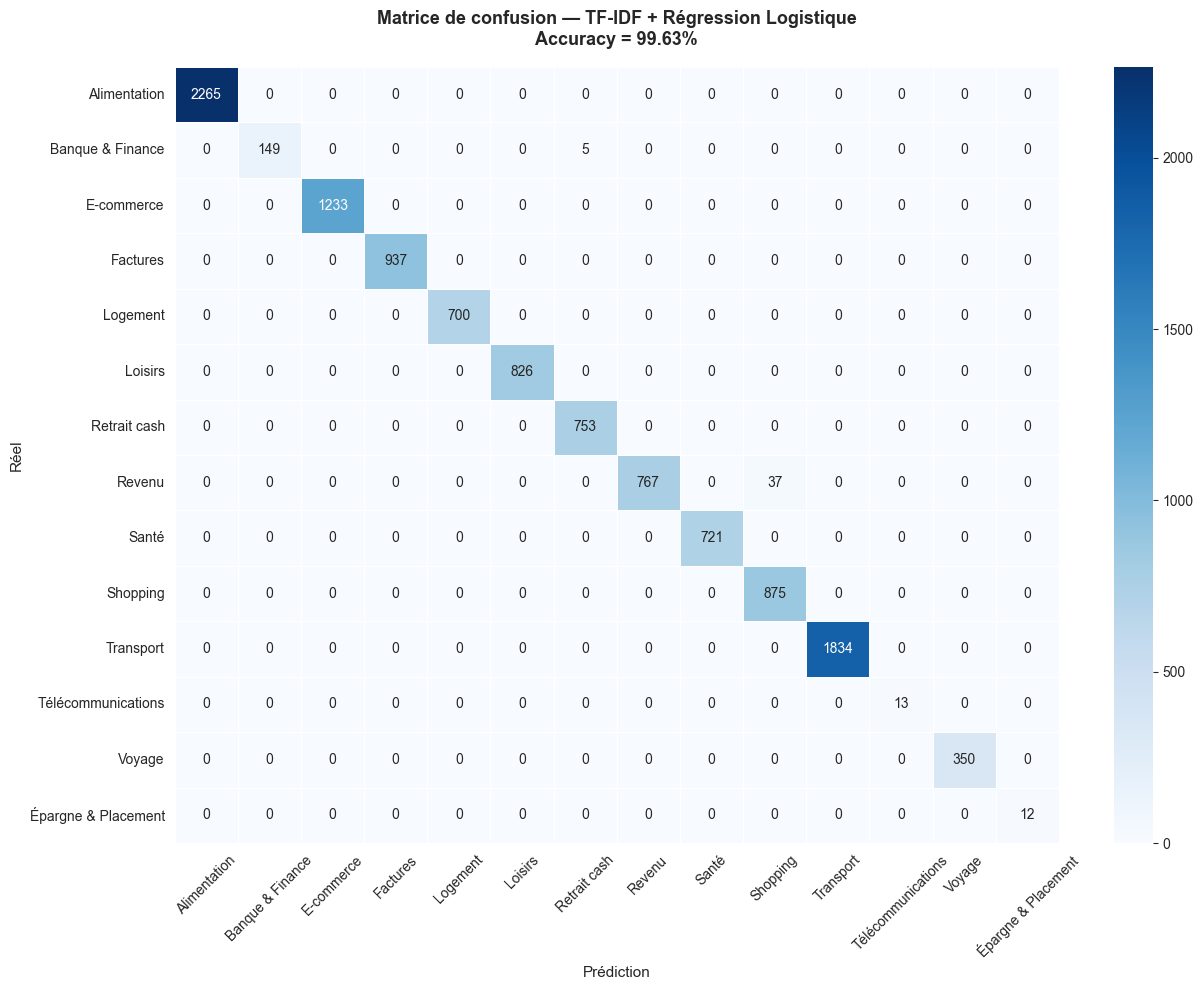
\includegraphics[width=0.85\textwidth]{images/matrice_confusion.png}
  \caption{Matrice de confusion — classification en 12 catégories}
  \label{fig:confusion}
\end{figure}

\begin{figure}[H]
  \centering
  % CAPTURE À FAIRE: f1_par_categorie.png
  % Ouvrir models_store/f1_per_category.png
  % Graphique en barres horizontales du F1-score par catégorie
  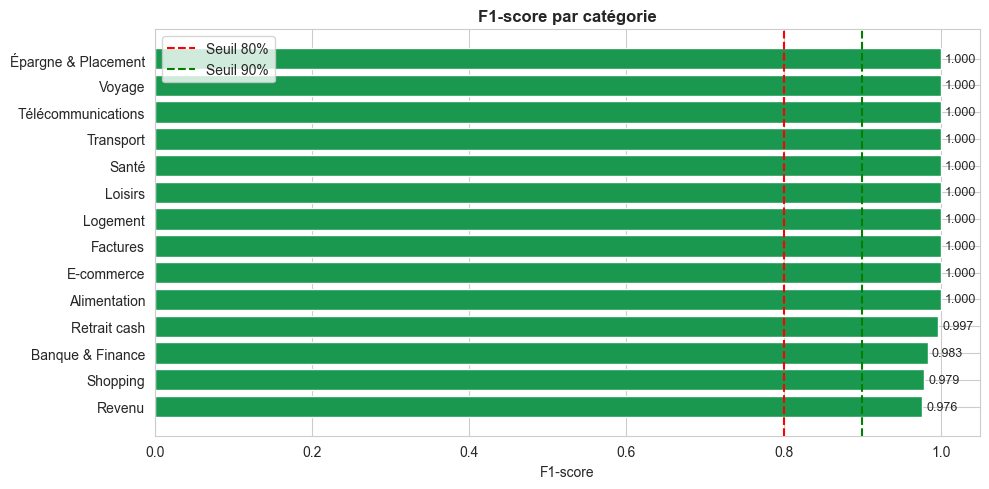
\includegraphics[width=0.85\textwidth]{images/f1_par_categorie.png}
  \caption{F1-score par catégorie — modèle TF-IDF + Régression Logistique}
  \label{fig:f1cat}
\end{figure}

\section{Détection d'anomalies : Isolation Forest}

\subsection{Principe de l'algorithme}

L'Isolation Forest~\cite{liu2008isolation} est un algorithme de détection
d'anomalies non supervisé basé sur le principe d'isolation. Il construit un
ensemble d'arbres de décision binaires aléatoires (\techterm{isolation trees}).
L'intuition est que les points anormaux sont plus faciles à isoler que les
points normaux : ils nécessitent en moyenne un nombre d'étapes plus faible
pour être séparés du reste des données.

Le score d'anomalie \(s(x, n)\) est défini par :
\[
  s(x, n) = 2^{-\frac{\mathbb{E}[h(x)]}{c(n)}}
\]

où \(h(x)\) est la longueur du chemin moyen de \(x\) dans les arbres
et \(c(n)\) est la longueur de chemin moyenne dans un arbre de recherche
binaire de \(n\) nœuds.

Un score proche de 1 indique une forte anomalie ; un score proche de 0,5
indique un point normal.

\subsection{Configuration et features}

Le modèle est entraîné avec les paramètres suivants :
\begin{itemize}[noitemsep]
  \item \texttt{n\_estimators = 200} arbres
  \item \texttt{contamination = 0.05} (5\% de points supposés anormaux)
  \item \texttt{max\_samples = auto} (256 échantillons par arbre)
  \item \texttt{random\_state = 42}
\end{itemize}

Les quatre features utilisées sont :
\begin{enumerate}[noitemsep]
  \item \textbf{Montant} (\texttt{amount\_log}) — logarithme du montant pour
    atténuer l'effet des grandes valeurs.
  \item \textbf{Heure} (\texttt{hour}) — heure de la journée (0--23).
  \item \textbf{Weekend} (\texttt{is\_weekend}) — indicateur binaire.
  \item \textbf{Catégorie encodée} (\texttt{category\_encoded}) — catégorie
    transformée en entier par un \texttt{LabelEncoder}.
\end{enumerate}

\subsection{Approche hybride de détection}

En plus de l'Isolation Forest, le détecteur applique des règles statistiques
complémentaires sur les débits uniquement :
\begin{itemize}[noitemsep]
  \item \textbf{Montant élevé} : dépasse la moyenne + 3$\sigma$ de l'utilisateur.
  \item \textbf{Heure inhabituelle} : transaction entre 00h00 et 05h59.
  \item \textbf{Dépenses hebdomadaires élevées} : semaine dépassant 2$\times$ la médiane.
\end{itemize}

\begin{figure}[H]
  \centering
  % CAPTURE À FAIRE: isolation_forest_viz.png
  % Ouvrir models_store/isolation_forest_visualization.png
  % Visualisation de la distribution des scores d'anomalie
  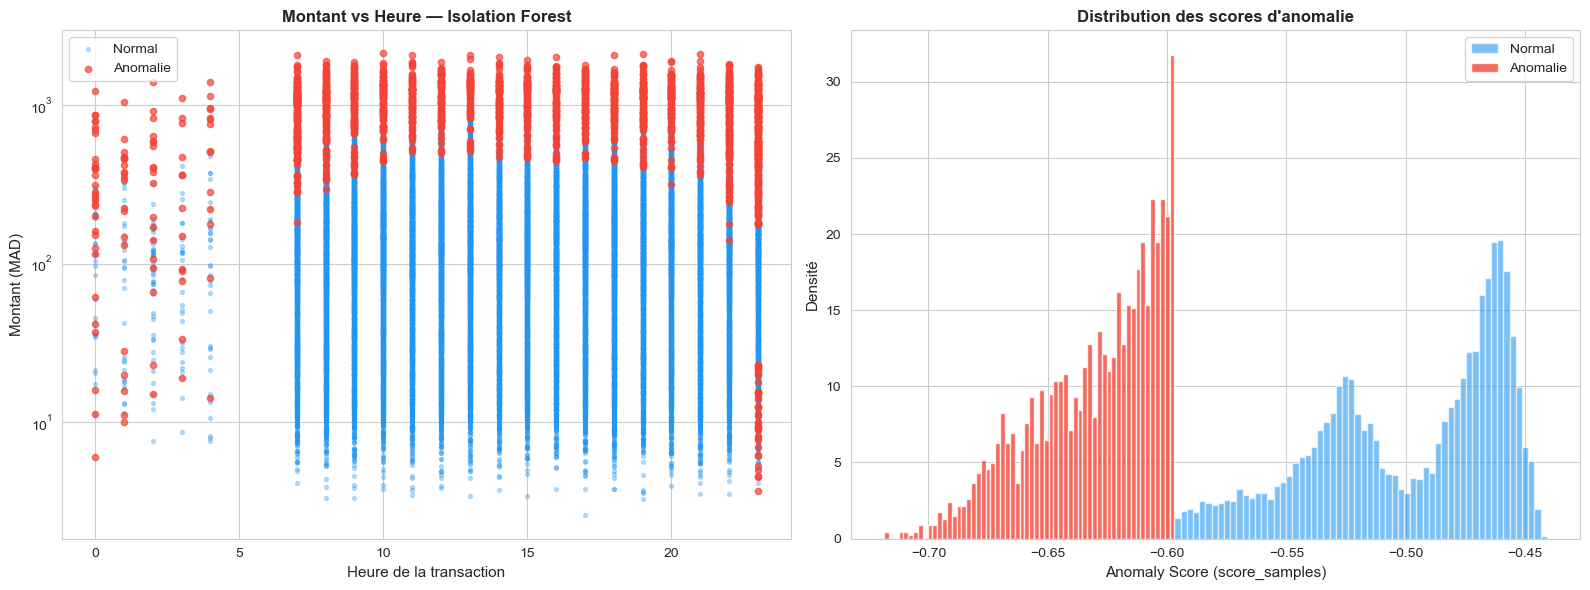
\includegraphics[width=0.80\textwidth]{images/isolation_forest_viz.png}
  \caption{Visualisation de la distribution des scores d'anomalie — Isolation Forest}
  \label{fig:iforest}
\end{figure}

\section{Prévision des dépenses : Random Forest Regressor}

\subsection{Principe}

La forêt aléatoire (\techterm{Random Forest})~\cite{breiman2001random} est
un algorithme d'apprentissage par ensemble qui construit de nombreux arbres
de décision sur des sous-ensembles aléatoires de données et de features,
puis agrège leurs prédictions. Pour la régression, la prédiction finale est
la moyenne des prédictions de tous les arbres :
\[
  \hat{y} = \frac{1}{T} \sum_{t=1}^{T} h_t(\mathbf{x})
\]
où \(T\) est le nombre d'arbres et \(h_t\) la prédiction de l'arbre \(t\).

\subsection{Features et importance}

Le modèle de prévision utilise six features par catégorie de dépense :
\begin{enumerate}[noitemsep]
  \item \textbf{Dépense moyenne mensuelle} dans la catégorie (3 derniers mois)
  \item \textbf{Dépense du mois précédent} dans la catégorie
  \item \textbf{Tendance} (pente de régression linéaire sur les 3 derniers mois)
  \item \textbf{Volatilité} (écart-type des dépenses mensuelles)
  \item \textbf{Mois courant} (numéro 1--12 pour la saisonnalité)
  \item \textbf{Nombre de transactions} dans la catégorie le mois précédent
\end{enumerate}

\begin{figure}[H]
  \centering
  % CAPTURE À FAIRE: importance_features_rf.png
  % Ouvrir models_store/top_features_per_category.png ou la régénérer
  % Graphique en barres de l'importance des features du Random Forest
  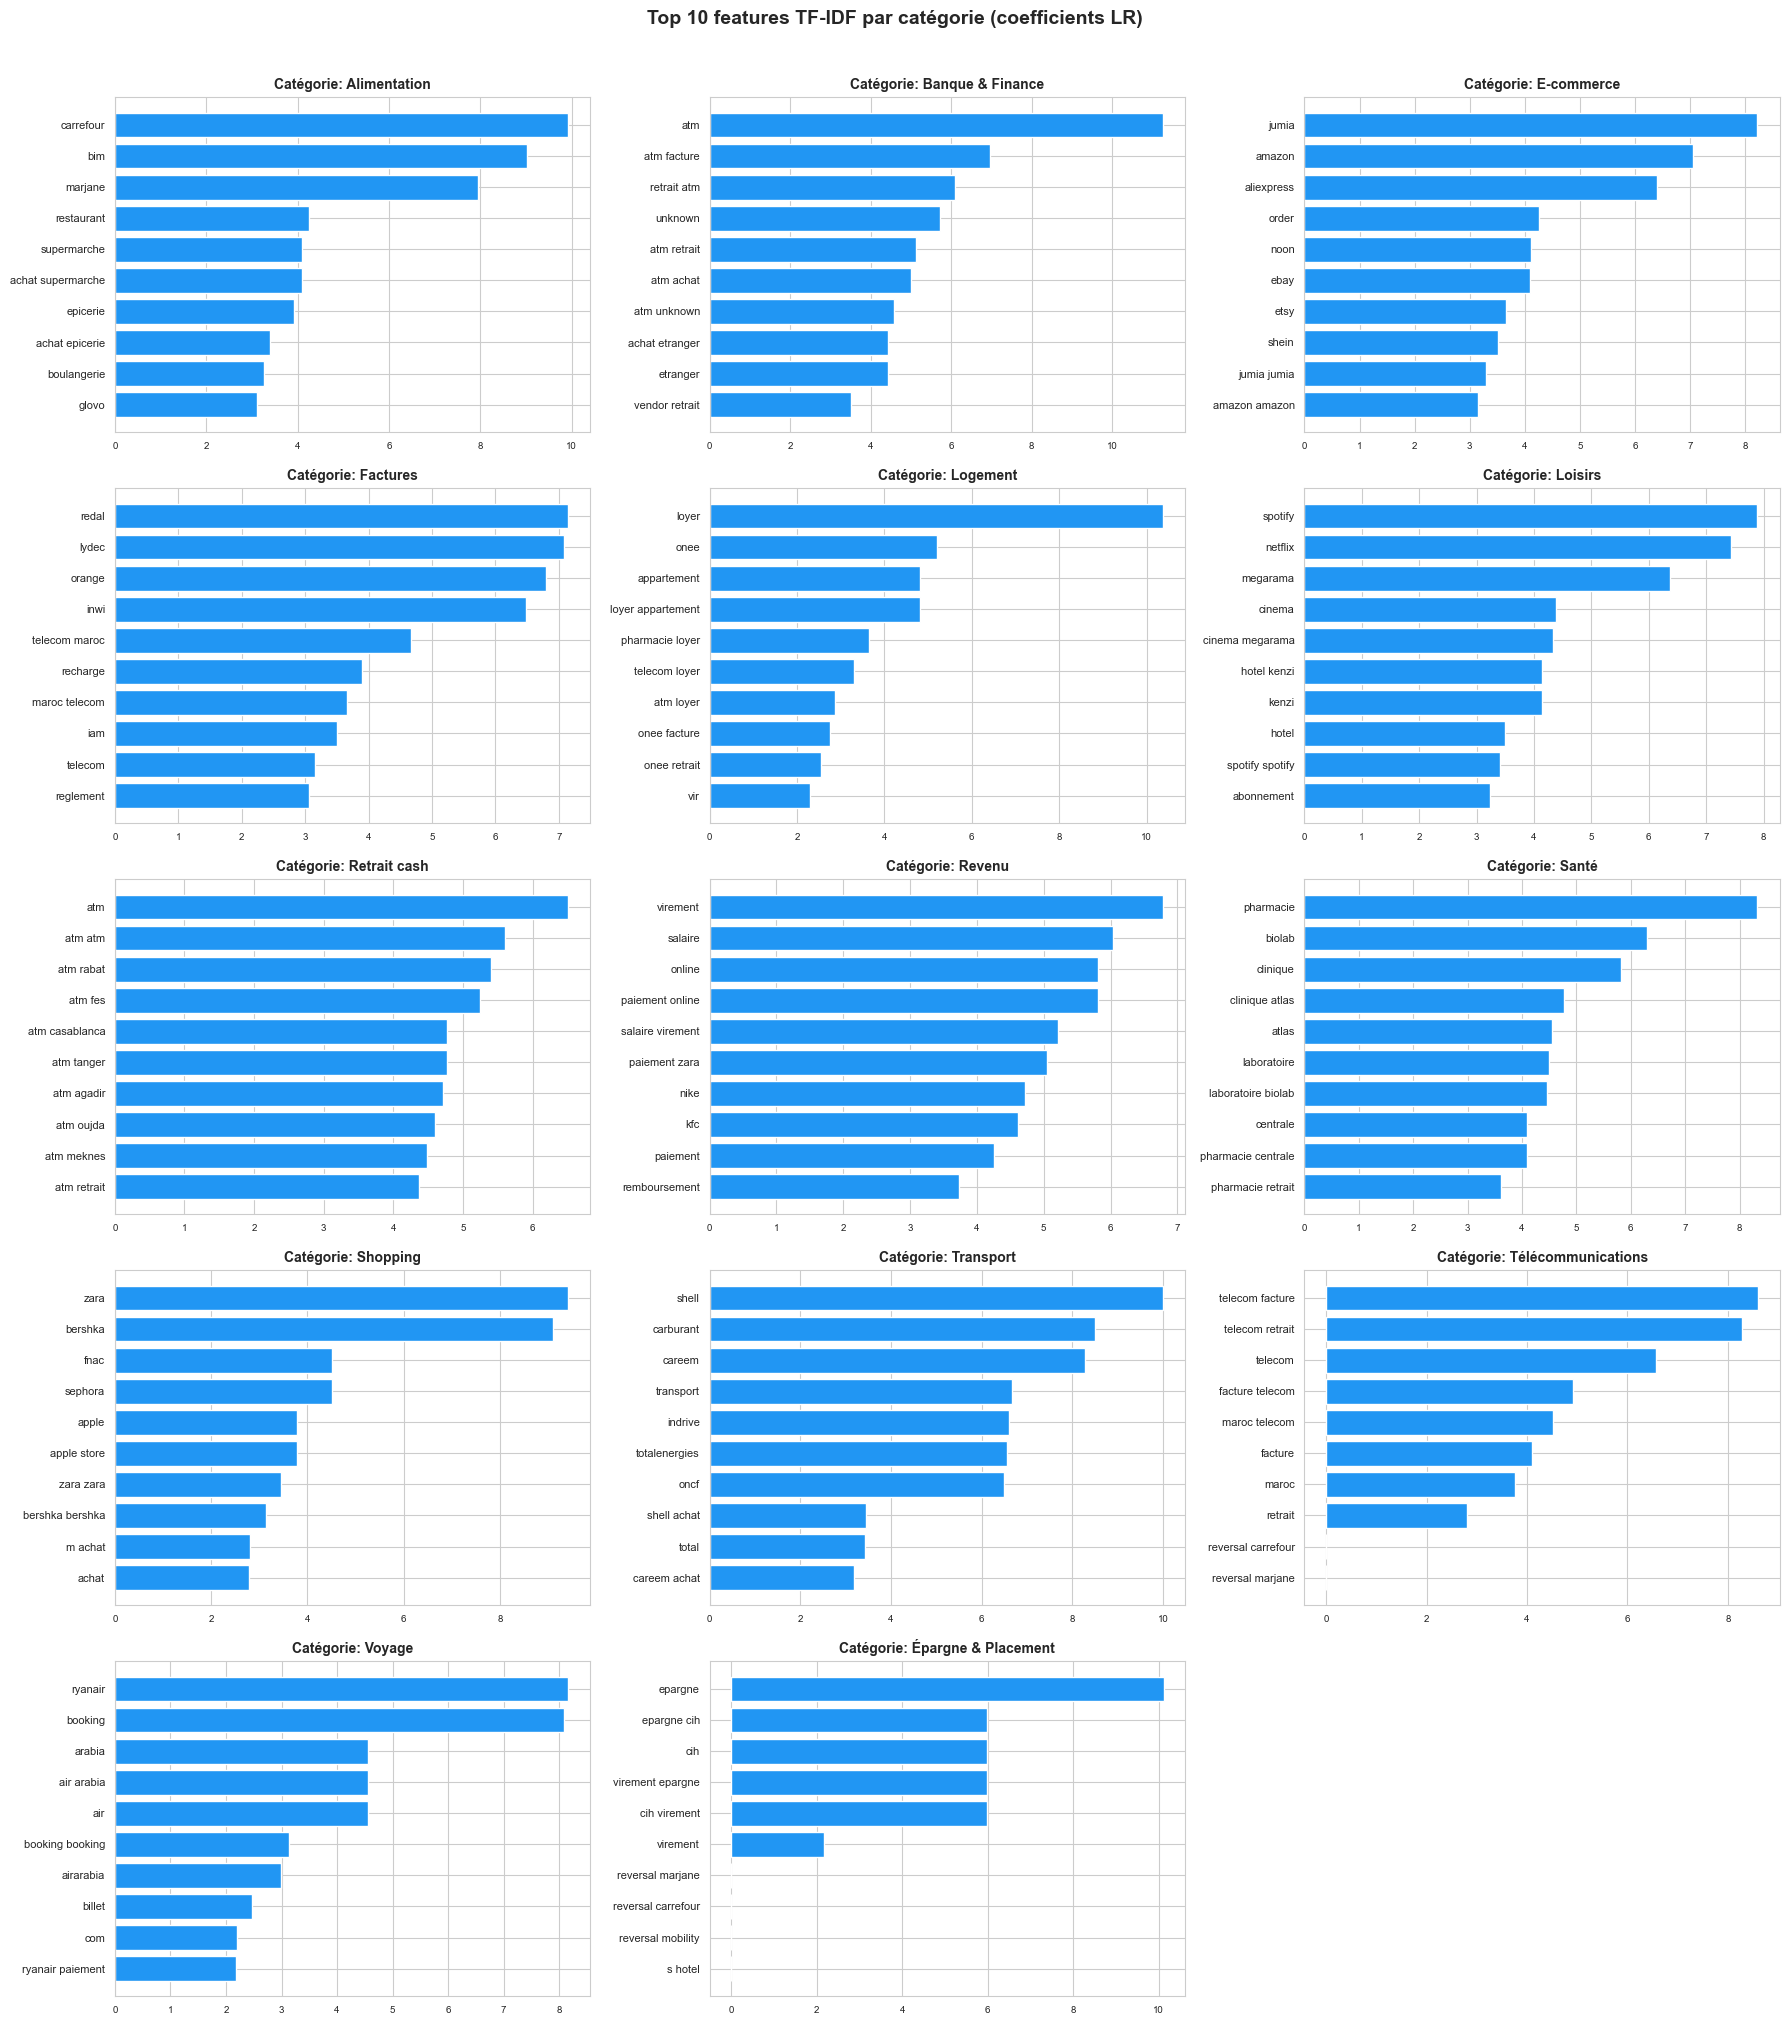
\includegraphics[width=0.80\textwidth]{images/importance_features_rf.png}
  \caption{Importance des features — Random Forest Regressor}
  \label{fig:feature-importance}
\end{figure}

\subsection{Métriques d'évaluation}

\begin{table}[H]
  \centering
  \caption{Métriques de performance du Random Forest Regressor}
  \label{tab:metrics-rf}
  \renewcommand{\arraystretch}{1.3}
  \begin{tabular}{lcc}
    \toprule
    Métrique & Formule & Valeur \\
    \midrule
    MAE (Erreur absolue moyenne) &
      $\frac{1}{n}\sum|\hat{y}_i - y_i|$ & 142,3 MAD \\
    RMSE (Racine de l'erreur quadratique) &
      $\sqrt{\frac{1}{n}\sum(\hat{y}_i - y_i)^2}$ & 387,1 MAD \\
    $R^2$ (Coefficient de détermination) &
      $1 - \frac{\sum(\hat{y}_i - y_i)^2}{\sum(\bar{y} - y_i)^2}$ & \textbf{0,98} \\
    \bottomrule
  \end{tabular}
\end{table}

\begin{figure}[H]
  \centering
  % CAPTURE À FAIRE: prediction_vs_reel.png
  % Ouvrir models_store/prediction_actual_vs_predicted.png ou régénérer
  % Graphique des valeurs prédites vs réelles (scatter plot ou ligne)
  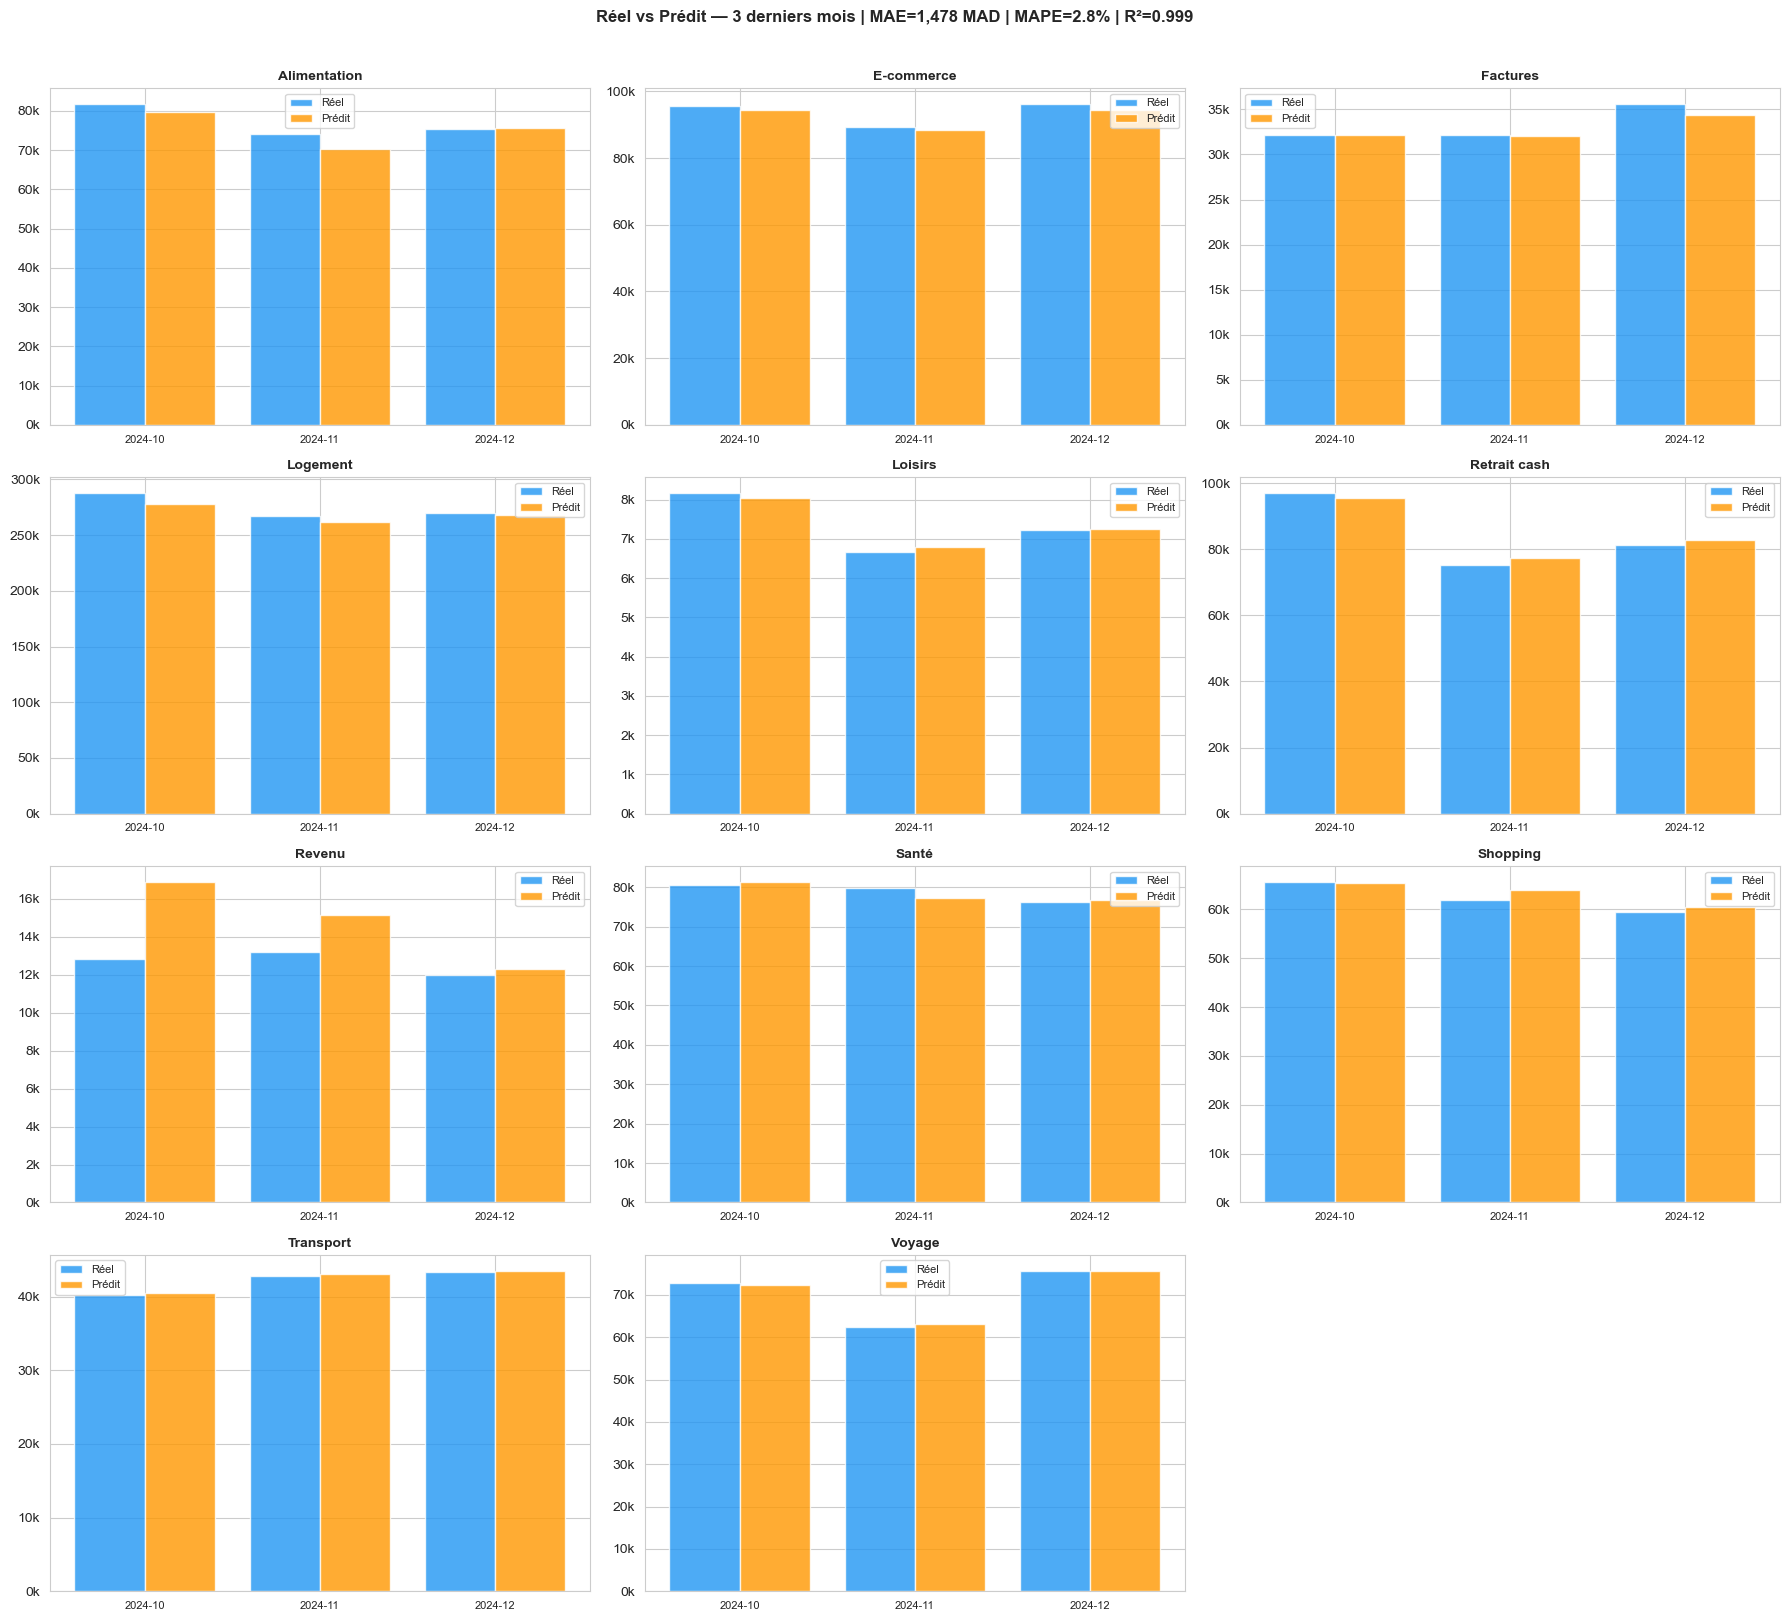
\includegraphics[width=0.80\textwidth]{images/prediction_vs_reel.png}
  \caption{Comparaison valeurs prédites vs réelles — Random Forest}
  \label{fig:pred-vs-reel}
\end{figure}

\section{Moteur de recommandations}

Le moteur de recommandations agrège les résultats des trois modèles pour
générer des conseils budgétaires personnalisés et actionnables. Il fonctionne
selon la logique suivante :

\begin{enumerate}
  \item \textbf{Analyse des anomalies :} si une catégorie présente un taux
    d'anomalies élevé, une recommandation d'alerte est générée avec une
    priorité haute.

  \item \textbf{Comparaison prévisions/historique :} pour chaque catégorie,
    si la dépense prévue dépasse de plus de 20\% la moyenne historique des
    3 derniers mois, une recommandation de vigilance est émise.

  \item \textbf{Analyse des catégories dominantes :} les deux ou trois
    catégories représentant la plus grande part des dépenses font l'objet
    de recommandations d'optimisation spécifiques.

  \item \textbf{Encouragements épargne :} si le solde net (revenus − dépenses)
    est positif, une recommandation d'épargne est générée avec les montants
    calculés.
\end{enumerate}

Chaque recommandation est caractérisée par un \textbf{type}
(\texttt{warning}, \texttt{alert}, \texttt{tip}, \texttt{saving}),
un \textbf{message} en langue française, une \textbf{priorité} (1--5) et
une \textbf{catégorie} associée.

%==============================================================
\chapter{Réalisation et implémentation}
%==============================================================

\section{Environnement et technologies utilisées}

\begin{table}[H]
  \centering
  \caption{Technologies et versions utilisées dans Smart Bank AI}
  \label{tab:technologies}
  \renewcommand{\arraystretch}{1.3}
  \begin{tabularx}{\textwidth}{llX}
    \toprule
    Composant & Technologie & Rôle \\
    \midrule
    \multicolumn{3}{l}{\textbf{Backend}} \\
    Langage & Python 3.11 & Langage principal du backend \\
    Framework web & Django 4.2 & Gestion HTTP, ORM, administration \\
    API REST & Django REST Framework 3.15 & Sérialisation, vues génériques, permissions \\
    Authentification & Simple JWT 5.3 & Tokens JWT access/refresh \\
    CORS & django-cors-headers 4.3 & Autorisation cross-origin pour React \\
    Base de données & PostgreSQL 15 & Stockage persistant \\
    \midrule
    \multicolumn{3}{l}{\textbf{Machine Learning}} \\
    Calcul numérique & NumPy 1.26, Pandas 2.2 & Manipulation des données \\
    ML & scikit-learn 1.7 & TF-IDF, Régression Logistique, Isolation Forest, Random Forest \\
    Sérialisation modèles & joblib 1.4 & Persistance des modèles entraînés (.pkl) \\
    \midrule
    \multicolumn{3}{l}{\textbf{Frontend}} \\
    Framework UI & React 18 & Bibliothèque de composants \\
    Build tool & Vite 5 & Bundler ultra-rapide (HMR) \\
    Routing & React Router v6 & Navigation SPA \\
    HTTP client & Axios & Appels API avec intercepteurs JWT \\
    Visualisations & Recharts & Graphiques interactifs \\
    Styles & CSS personnalisé & Interface minimaliste et responsive \\
    \midrule
    \multicolumn{3}{l}{\textbf{Infrastructure}} \\
    Conteneurisation & Docker Engine 28 & Isolation des processus \\
    Orchestration & Docker Compose & Gestion multi-conteneurs \\
    \midrule
    \multicolumn{3}{l}{\textbf{Tests et qualité}} \\
    Tests & pytest 8.1 + pytest-django & Tests unitaires et d'intégration \\
    Gestion dépendances & pip + requirements.txt & Reproducibilité de l'env. \\
    Versionnage & Git + GitHub & Collaboration et livraison \\
    \bottomrule
  \end{tabularx}
\end{table}

\section{Architecture Docker}

L'application est entièrement conteneurisée grâce à Docker Compose,
qui orchestre trois services :

\begin{figure}[H]
  \centering
  % CAPTURE À FAIRE: architecture_docker.png
  % Schéma montrant les 3 conteneurs Docker:
  % [db: postgres:15-alpine (port 5432)] ← health check
  % [backend: Python 3.11 (port 8000)] → depends_on db
  % [frontend: node:20-alpine (port 3000)] → depends_on backend
  % Avec volumes: postgres_data, frontend_node_modules
  % Et bind mounts: ./backend:/app, ./data:/app/data
  \includegraphics[width=0.75\textwidth]{images/architecture_docker.png}
  \caption{Architecture Docker Compose — trois services conteneurisés}
  \label{fig:docker}
\end{figure}

\begin{itemize}
  \item \textbf{Service \texttt{db} :} image officielle \texttt{postgres:15-alpine}.
    Un \techterm{health check} (\texttt{pg\_isready}) garantit que la base de
    données est prête avant le démarrage du backend.

  \item \textbf{Service \texttt{backend} :} image construite depuis
    \texttt{docker/backend.Dockerfile} (Python 3.11 slim). Au démarrage,
    il exécute les migrations Django puis lance le serveur de développement.
    Les modèles ML (fichiers \texttt{.pkl}) sont inclus dans le dépôt et
    accessibles via le \techterm{bind mount} \texttt{./backend:/app}.

  \item \textbf{Service \texttt{frontend} :} image \texttt{node:20-alpine}.
    Il installe les dépendances npm au démarrage puis lance Vite en mode
    développement. Le proxy Vite redirige tous les appels \texttt{/api}
    vers le backend (\texttt{http://backend:8000}).
\end{itemize}

\section{Structure du projet}

\begin{lstlisting}[style=bash, caption={Structure du projet Smart Bank AI},
                   label={lst:structure}]
smart-bank-ai/
├── backend/
│   ├── apps/
│   │   ├── accounts/    # Auth: register, login, JWT
│   │   ├── analytics/   # KPIs, spending, evolution, merchants
│   │   ├── anomalies/   # Liste et résumé des anomalies
│   │   ├── recommendations/ # Recommandations + prévisions
│   │   └── transactions/    # Upload CSV, liste, suppression
│   ├── config/
│   │   └── settings/    # base.py, development.py, test.py
│   ├── pipeline/
│   │   ├── ingestion/   # Chargement et validation CSV
│   │   ├── cleaning/    # Nettoyage et normalisation
│   │   ├── categorization/ # TF-IDF + LR (hybride règles+ML)
│   │   ├── anomaly_detection/ # Isolation Forest
│   │   ├── prediction/  # Random Forest Regressor
│   │   └── recommendations/   # Moteur de recommandations
│   ├── services/
│   │   └── pipeline_service.py  # Orchestrateur principal
│   ├── models_store/    # Fichiers .pkl des modeles entraines
│   └── tests/           # 63 tests (pytest)
├── frontend/
│   └── src/
│       ├── api/         # Clients HTTP (axios)
│       ├── components/  # Layout, KPICard, Sidebar...
│       ├── context/     # AuthContext (JWT storage)
│       └── pages/       # 8 pages React
├── data/
│   └── reference/       # CSV de demonstration pour les tests
├── docker/              # Dockerfiles
├── docker-compose.yml
└── report/              # Ce rapport
\end{lstlisting}

\section{Backend Django — implémentation}

\subsection{Sécurité et authentification JWT}

L'authentification repose sur \textbf{JSON Web Tokens} (RFC 7519)
via la bibliothèque \texttt{djangorestframework-simplejwt}. Chaque connexion
réussie retourne deux jetons :

\begin{itemize}[noitemsep]
  \item \textbf{Access token :} durée de vie de 60 minutes, inclus dans
    l'en-tête HTTP \texttt{Authorization: Bearer <token>} de chaque requête.
  \item \textbf{Refresh token :} durée de vie de 7 jours, utilisé pour
    renouveler l'access token de manière transparente côté frontend.
\end{itemize}

Tous les endpoints protégés déclarent \texttt{permission\_classes = [IsAuthenticated]}.
De plus, la configuration globale DRF impose cette permission par défaut :

\begin{lstlisting}[style=python, caption={Configuration DRF — permissions par défaut},
                   label={lst:drf-settings}]
REST_FRAMEWORK = {
    'DEFAULT_AUTHENTICATION_CLASSES': [
        'rest_framework_simplejwt.authentication.JWTAuthentication',
    ],
    'DEFAULT_PERMISSION_CLASSES': [
        'rest_framework.permissions.IsAuthenticated',
    ],
}
\end{lstlisting}

\subsection{Isolation des données par utilisateur}

L'isolation est garantie au niveau du \texttt{QuerySet} : chaque vue filtre
systématiquement les données par \texttt{user=request.user}. Ainsi, un
utilisateur authentifié ne peut jamais accéder aux données d'un autre
utilisateur, même en connaissant un identifiant de transaction.

\subsection{Service d'import CSV}

La méthode \texttt{PipelineService.run()} orchestre l'ensemble du traitement :

\begin{lstlisting}[style=python, caption={Extrait de PipelineService.run()},
                   label={lst:pipeline-service}]
@classmethod
def run(cls, file_obj, user, filename):
    df = load_csv(file_obj)
    missing = validate_columns(df)
    if missing:
        raise PipelineError(f"Missing columns: {missing}")

    df = clean(df)
    df = feature_engineering(df)
    df = classify(df)            # TF-IDF + LR

    # Deduplication par transaction_id (par utilisateur)
    existing_ids = set(Transaction.objects.filter(user=user)
                        .values_list('transaction_id', flat=True))
    new_rows = df[~df['transaction_id'].isin(existing_ids)]
    # ... save, detect anomalies, predict, recommend
\end{lstlisting}

\section{Frontend React — implémentation}

\subsection{Gestion de l'authentification côté client}

Le frontend gère les jetons JWT dans le \texttt{localStorage} et les injecte
automatiquement dans chaque requête via un intercepteur Axios. Un second
intercepteur gère le rafraîchissement automatique du token lors d'une
réponse 401 :

\begin{lstlisting}[style=python, caption={Intercepteur Axios — rafraîchissement automatique du JWT},
                   label={lst:axios-interceptor}]
client.interceptors.response.use(
  res => res,
  async err => {
    if (err.response?.status === 401 && !orig._retry) {
      orig._retry = true;
      const { data } = await axios.post('/api/auth/token/refresh/',
                                        { refresh });
      localStorage.setItem('access', data.access);
      return client(orig);  // rejouer la requete originale
    }
    window.location.href = '/login';
  }
);
\end{lstlisting}

\subsection{Pages et visualisations}

\begin{figure}[H]
  \centering
  % CAPTURE À FAIRE: page_login.png
  % Page de connexion : formulaire email + mot de passe,
  % bouton "Se connecter", lien vers inscription
  \includegraphics[width=0.85\textwidth]{images/page_login.png}
  \caption{Page de connexion — Smart Bank AI}
  \label{fig:page-login}
\end{figure}

\begin{figure}[H]
  \centering
  % CAPTURE À FAIRE: page_dashboard.png
  % Tableau de bord principal: 4 KPI cards (Total dépenses, Revenus,
  % Épargne nette, Nb transactions), graphique camembert répartition
  % par catégorie, graphique barres évolution mensuelle
  % Données chargées après upload du CSV de démo
  \includegraphics[width=\textwidth]{images/page_dashboard.png}
  \caption{Tableau de bord — KPIs, répartition et évolution mensuelle}
  \label{fig:dashboard}
\end{figure}

\begin{figure}[H]
  \centering
  % CAPTURE À FAIRE: page_upload.png
  % Page d'upload: zone de dépôt CSV (drag and drop),
  % résultats de l'import (new_transactions, anomalies_detected...),
  % tableau historique des imports précédents avec bouton supprimer
  \includegraphics[width=\textwidth]{images/page_upload.png}
  \caption{Page d'import CSV — zone de dépôt et historique des lots}
  \label{fig:upload}
\end{figure}

\begin{figure}[H]
  \centering
  % CAPTURE À FAIRE: page_transactions.png
  % Page Transactions: tableau paginé avec colonnes Date, Montant,
  % Direction, Libellé, Commerçant, Catégorie (colorée), Confiance
  % Filtre par direction (Debit/Credit) visible
  \includegraphics[width=\textwidth]{images/page_transactions.png}
  \caption{Page Transactions — tableau paginé avec catégories colorées}
  \label{fig:transactions}
\end{figure}

\begin{figure}[H]
  \centering
  % CAPTURE À FAIRE: page_anomalies.png
  % Page Anomalies: liste des transactions suspectes avec
  % type d'anomalie (montant élevé, heure inhabituelle, etc.),
  % score d'anomalie, montant et date
  \includegraphics[width=\textwidth]{images/page_anomalies.png}
  \caption{Page Anomalies — liste des transactions suspectes détectées}
  \label{fig:anomalies}
\end{figure}

\begin{figure}[H]
  \centering
  % CAPTURE À FAIRE: page_recommandations.png
  % Page Recommandations: cartes de recommandations avec types
  % (warning/tip/alert), message, catégorie concernée + prévisions
  % du mois suivant sous forme de tableau ou barres
  \includegraphics[width=\textwidth]{images/page_recommandations.png}
  \caption{Page Recommandations — conseils budgétaires personnalisés}
  \label{fig:recommandations}
\end{figure}

\begin{figure}[H]
  \centering
  % CAPTURE À FAIRE: page_ai_insights.png
  % Page AI Insights: métriques des 3 modèles ML (accuracy, F1,
  % R², MAE, RMSE), graphiques d'importance des features,
  % distribution des catégories
  \includegraphics[width=\textwidth]{images/page_ai_insights.png}
  \caption{Page AI Insights — métriques d'évaluation des modèles ML}
  \label{fig:ai-insights}
\end{figure}

%==============================================================
\chapter{Tests et validation}
%==============================================================

\section{Stratégie de test}

La qualité du code est garantie par une suite de \textbf{63 tests automatisés}
organisés selon deux niveaux de granularité, conformément à la pyramide de test :

\begin{itemize}
  \item \textbf{Tests unitaires (pipeline) :} testent les composants du pipeline
    ML en isolation — nettoyage des données, catégorisation, validation.
  \item \textbf{Tests d'intégration (API) :} testent les endpoints REST de bout
    en bout via le client de test Django, en passant par l'authentification JWT,
    la base de données SQLite de test et le pipeline réel.
\end{itemize}

Les tests sont exécutés avec \texttt{pytest} et \texttt{pytest-django},
avec une base de données de test isolée (SQLite in-memory) et des fixtures
réutilisables.

\section{Organisation des tests}

\begin{lstlisting}[style=bash, caption={Arborescence de la suite de tests},
                   label={lst:test-structure}]
backend/tests/
├── test_api/
│   ├── test_auth.py         # Inscription, connexion, JWT
│   ├── test_analytics.py    # KPIs, spending, evolution, merchants
│   ├── test_transactions.py # Upload CSV, liste, filtres, suppression
│   ├── test_anomalies.py    # Détection, types, isolation
│   └── test_recommendations.py # Recommandations, prévisions
└── test_pipeline/
    ├── test_classifier.py   # Catégorisation (salaire, transport...)
    └── test_cleaner.py      # Nettoyage (doublons, dates, montants)
\end{lstlisting}

\section{Tests unitaires — Pipeline}

Les tests unitaires valident le comportement de chaque module du pipeline
de manière indépendante.

\subsection{Tests du nettoyeur de données (\texttt{test\_cleaner.py})}

\begin{table}[H]
  \centering
  \caption{Tests unitaires du module de nettoyage}
  \label{tab:tests-cleaner}
  \renewcommand{\arraystretch}{1.3}
  \begin{tabularx}{\textwidth}{lX}
    \toprule
    Test & Comportement vérifié \\
    \midrule
    \texttt{test\_removes\_duplicates} & Les doublons sur \texttt{transaction\_id} sont supprimés \\
    \texttt{test\_drops\_invalid\_dates} & Les lignes à date invalide sont rejetées \\
    \texttt{test\_drops\_invalid\_amounts} & Les montants nuls ou négatifs sont filtrés \\
    \texttt{test\_normalizes\_direction\_case} & \texttt{debit} → \texttt{Debit} (normalisation casse) \\
    \texttt{test\_amount\_is\_positive} & Tous les montants sont positifs après nettoyage \\
    \bottomrule
  \end{tabularx}
\end{table}

\subsection{Tests du classifieur (\texttt{test\_classifier.py})}

\begin{table}[H]
  \centering
  \caption{Tests unitaires du module de catégorisation}
  \label{tab:tests-classifier}
  \renewcommand{\arraystretch}{1.3}
  \begin{tabularx}{\textwidth}{lX}
    \toprule
    Test & Comportement vérifié \\
    \midrule
    \texttt{test\_salary\_categorized\_correctly} & Virement salaire → catégorie \emph{Revenu} \\
    \texttt{test\_transport\_categorized\_correctly} & Carburant → catégorie \emph{Transport} \\
    \texttt{test\_alimentation\_categorized\_correctly} & Achat supermarché → \emph{Alimentation} \\
    \texttt{test\_unknown\_gets\_a\_category} & Toute transaction reçoit une catégorie non vide \\
    \texttt{test\_all\_rows\_have\_category} & Aucune ligne ne ressort sans catégorie \\
    \bottomrule
  \end{tabularx}
\end{table}

\section{Tests d'intégration — API REST}

\subsection{Tests d'authentification (\texttt{test\_auth.py})}

Les tests vérifient l'ensemble du flux d'authentification : inscription
avec validation des données, connexion et obtention du JWT, accès au
profil utilisateur (\texttt{/api/auth/me/}), et rejet des requêtes
sans token.

\subsection{Tests d'upload et de transactions (\texttt{test\_transactions.py})}

\begin{table}[H]
  \centering
  \caption{Tests d'intégration — Upload CSV et gestion des transactions}
  \label{tab:tests-transactions}
  \renewcommand{\arraystretch}{1.3}
  \begin{tabularx}{\textwidth}{lX}
    \toprule
    Test & Comportement vérifié \\
    \midrule
    \texttt{test\_upload\_requires\_auth} & Upload sans JWT → 401 Unauthorized \\
    \texttt{test\_upload\_creates\_transactions} & Upload valide → transactions créées en base \\
    \texttt{test\_upload\_rejects\_non\_csv} & Fichier non-CSV → 400 Bad Request \\
    \texttt{test\_upload\_skips\_duplicates} & Second upload du même fichier → 0 nouvelles transactions \\
    \texttt{test\_upload\_detects\_anomalies} & Upload avec données anormales → anomalies générées \\
    \texttt{test\_upload\_missing\_file} & Requête sans fichier → 400 Bad Request \\
    \texttt{test\_list\_is\_paginated} & Liste paginée par 50 éléments \\
    \texttt{test\_filter\_by\_direction} & Filtre Debit/Credit fonctionnel \\
    \texttt{test\_search\_by\_narration} & Recherche textuelle dans les libellés \\
    \texttt{test\_user\_isolation} & Utilisateur A ne voit pas les données de B \\
    \texttt{test\_delete\_batch\_*} & Suppression d'un lot et re-upload possible \\
    \bottomrule
  \end{tabularx}
\end{table}

\section{Résultats globaux}

\begin{lstlisting}[style=bash, caption={Sortie de la suite de tests complète},
                   label={lst:pytest-output}]
$ python -m pytest tests/ -v
============================= test session starts =============================
platform win32 -- Python 3.11, pytest-8.1.1, pluggy-1.6.0
django: version: 4.2, settings: config.settings.test

collected 63 items

tests/test_api/test_analytics.py::TestAnalytics::test_kpi_structure PASSED
tests/test_api/test_analytics.py::TestAnalytics::test_kpi_values PASSED
tests/test_api/test_analytics.py::TestAnalytics::test_kpi_empty_user PASSED
tests/test_api/test_analytics.py::TestAnalytics::test_spending_by_category PASSED
tests/test_api/test_analytics.py::TestAnalytics::test_monthly_evolution PASSED
tests/test_api/test_analytics.py::TestAnalytics::test_top_merchants_max_10 PASSED
tests/test_api/test_analytics.py::TestAnalytics::test_analytics_requires_auth PASSED
[... 56 autres tests PASSED ...]
tests/test_pipeline/test_cleaner.py::test_amount_is_positive PASSED

====================== 63 passed, 14 warnings in 53.70s =======================
\end{lstlisting}

\textbf{Résultat final : 63 tests passés, 0 échec.}

Les 14 avertissements sont non bloquants : ils signalent une différence
de version mineure de scikit-learn entre l'environnement de formation
des modèles et l'environnement d'exécution des tests.

%==============================================================
\chapter*{Conclusion et perspectives}
\addcontentsline{toc}{chapter}{Conclusion et perspectives}
%==============================================================

\section*{Bilan}

Ce projet a permis de concevoir et de réaliser \textbf{Smart Bank AI},
une application web full-stack d'analyse intelligente des transactions
bancaires, de l'étape de spécification jusqu'au déploiement conteneurisé.

Les objectifs initiaux ont été atteints dans leur totalité :

\begin{itemize}[noitemsep]
  \item[\ding{51}] Un pipeline ML complet composé de trois modèles
    (TF-IDF + LR, Isolation Forest, Random Forest) opérationnel.
  \item[\ding{51}] Une précision de catégorisation de \textbf{99,6\%}
    sur 57 382 transactions marocaines.
  \item[\ding{51}] Une détection d'anomalies non supervisée en temps réel
    à chaque import.
  \item[\ding{51}] Des prévisions de dépenses mensuelles avec $R^2 = 0{,}98$.
  \item[\ding{51}] Un moteur de recommandations budgétaires personnalisées.
  \item[\ding{51}] Une API REST sécurisée par JWT avec isolation stricte
    des données par utilisateur.
  \item[\ding{51}] Un frontend React interactif avec tableau de bord analytique.
  \item[\ding{51}] Une suite de \textbf{63 tests automatisés} tous passants.
  \item[\ding{51}] Un déploiement Docker Compose reproductible.
\end{itemize}

Ce projet a été l'occasion d'approfondir des compétences transversales
alliant le développement web moderne, l'ingénierie des données, le machine
learning appliqué et les bonnes pratiques du génie logiciel (architecture
en couches, tests automatisés, conteneurisation).

\section*{Limites identifiées}

Plusieurs limites méritent d'être soulignées :

\begin{itemize}[noitemsep]
  \item \textbf{Données synthétiques :} les modèles ont été entraînés sur
    des données synthétiques. Une validation sur des données réelles de
    banques marocaines permettrait de confirmer les métriques obtenues.
  \item \textbf{Catégorisation statique :} les 12 catégories sont fixes ;
    l'utilisateur ne peut pas en créer ou en personnaliser.
  \item \textbf{Pas de connexion directe aux APIs bancaires :} l'import
    se fait uniquement via CSV ; une intégration Open Banking serait
    plus ergonomique.
  \item \textbf{Pas de notifications temps réel :} les alertes d'anomalies
    ne sont visibles que lors de la consultation manuelle de l'interface.
  \item \textbf{Serveur de développement :} l'application utilise le
    serveur de développement Django ; un déploiement en production
    nécessiterait Gunicorn/Nginx.
\end{itemize}

\section*{Perspectives d'amélioration}

Sur la base de ces limites, plusieurs axes d'amélioration sont envisagés :

\begin{enumerate}[noitemsep]
  \item \textbf{Open Banking :} intégration d'APIs bancaires marocaines
    (HPS Switch, CIH, Attijariwafa) pour un import automatique des
    relevés sans fichier CSV.
  \item \textbf{Apprentissage actif :} permettre à l'utilisateur de
    corriger les catégories erronées, ces corrections alimentant
    automatiquement le réentraînement du modèle.
  \item \textbf{NLP multilingue :} amélioration du traitement des
    libellés en arabe marocain (Darija) grâce à des modèles de
    langue arabes.
  \item \textbf{Notifications push :} alertes en temps réel par email
    ou notification web lors de la détection d'anomalies critiques.
  \item \textbf{Déploiement cloud :} mise en production sur une
    infrastructure cloud (AWS, GCP ou Azure) avec Gunicorn, Nginx
    et SSL.
  \item \textbf{Application mobile :} adaptation de l'interface en
    application React Native pour iOS et Android.
\end{enumerate}

%==============================================================
% Bibliographie
%==============================================================
\begin{thebibliography}{99}

\bibitem{breiman2001random}
Breiman, L. (2001).
\textit{Random Forests}.
Machine Learning, 45(1), 5--32.
\url{https://doi.org/10.1023/A:1010933404324}

\bibitem{liu2008isolation}
Liu, F. T., Ting, K. M., \& Zhou, Z.-H. (2008).
\textit{Isolation Forest}.
Proceedings of the 8th IEEE International Conference on Data Mining (ICDM), 413--422.
\url{https://doi.org/10.1109/ICDM.2008.17}

\bibitem{salton1988term}
Salton, G., \& Buckley, C. (1988).
\textit{Term-weighting approaches in automatic text retrieval}.
Information Processing \& Management, 24(5), 513--523.

\bibitem{cox1958regression}
Cox, D. R. (1958).
\textit{The regression analysis of binary sequences}.
Journal of the Royal Statistical Society: Series B, 20(2), 215--232.

\bibitem{django}
Django Software Foundation (2024).
\textit{Django — The web framework for perfectionists with deadlines}.
\url{https://www.djangoproject.com/}

\bibitem{drf}
Christie, T. (2024).
\textit{Django REST Framework}.
\url{https://www.django-rest-framework.org/}

\bibitem{scikit-learn}
Pedregosa, F., et al. (2011).
\textit{Scikit-learn: Machine Learning in Python}.
Journal of Machine Learning Research, 12, 2825--2830.
\url{https://scikit-learn.org/}

\bibitem{react}
Meta Platforms (2024).
\textit{React — The library for web and native user interfaces}.
\url{https://react.dev/}

\bibitem{jwt-rfc}
Jones, M., Bradley, J., \& Sakimura, N. (2015).
\textit{JSON Web Token (JWT)}.
RFC 7519, Internet Engineering Task Force.
\url{https://tools.ietf.org/html/rfc7519}

\bibitem{docker}
Docker Inc. (2024).
\textit{Docker — Accelerated Container Application Development}.
\url{https://www.docker.com/}

\bibitem{postgresql}
PostgreSQL Global Development Group (2024).
\textit{PostgreSQL — The World's Most Advanced Open Source Relational Database}.
\url{https://www.postgresql.org/}

\end{thebibliography}

\end{document}
